\documentclass[a4paper]{article}
\usepackage[top=1in, left=1in]{geometry}
\usepackage{fancyhdr}
\usepackage{lastpage}
\usepackage{graphicx}
\usepackage{float}
\usepackage{amsmath}
\usepackage{amsfonts}
\usepackage{amssymb}
\usepackage{xcolor}
\usepackage{booktabs} % For table resizing
\usepackage{listings}
\usepackage{titling}

\renewcommand\maketitlehooka{\null\mbox{}\vfill}
\renewcommand\maketitlehookd{\vfill\null}

\pagestyle{fancy}
\fancyhf{}
\rhead{Econometrics Homework 3}
\lhead{Utpalraj Kemprai}

\cfoot{\thepage}

\begin{document}

\title{\huge Econometrics Homework 3}
\author{\LARGE Utpalraj Kemprai \\[5pt]
\LARGE MDS202352}
\date{}

\begin{titlingpage}
    \maketitle
\end{titlingpage}

\newpage

\section*{Question 1}

\(\displaystyle \theta \text{ is an unknown parameter satisfying } 0 \leq \theta \leq 1\). We have the following two experiments involving $\theta$.

\(\displaystyle \scalebox{1.5}{\ensuremath{\varepsilon}}_1 = \{Y_1, \theta, f_1 (y_1|\theta)\} \) is a binomial experiment in which a coin is flipped $T_1$ times, where $T_1$ is predetermined and $Y_1$ is the number of ``heads'' obtained in the $T_1$ flips.

\(\displaystyle \scalebox{1.5}{\ensuremath{\varepsilon}}_2 = \{Y_2, \theta, f_2 (y_2|\theta)\}\) is a negative binomial experiment in which a coin is flipped until m ``tails'' are obtained, where $m > 0$ is predetermined, and $Y_2$ is defined to be the number of ``heads'' obtained in the process.

\subsection*{Part (a)}

\noindent We assumes $\theta$ as the probability of the coin landing on head.

\noindent Clearly $Y_1$ follows a binomial distribution with parameters $T_1$ and $\theta$, i.e. $Y_1 \sim \text{Bin}(Y_1, \theta)$. So the p.m.f. for $Y_1$ is
\begin{align*}
    f_1(k|\theta,T_1) &= \begin{cases}
    \binom{T_1}{k} \times \theta^k (1 - \theta)^{T_1 - k} & \text{ if } 0 \leq k \leq T_1\\
    0 & \text{ otherwise }
        \end{cases}
\end{align*}

\noindent Now,

For $Y_2 = k, k \geq 0$, we must have $m-1$ tails and $k$ heads come up in $m+k-1$ tosses of the coin and a tail in the next toss i.e. $(m+k)^{\text{th}}$ toss of the coin.

The probability of getting $k$ heads in the first $m+k-1$ tosses of the coin is 
\begin{align*}
    P\left( k \text{ heads in }(m+k-1) \text{ tosses} \right) = \binom{m+k-1}{k} \times \theta^k (1-\theta)^{m-1}
\end{align*}

So the p.m.f. for $Y_2$ is

\begin{align*}
    f_2(k|\theta,m) &= P\left( k \text{ heads in }(m+k-1) \text{ tosses} \right)\times P\left( \text{tail in next toss} \right) \times I(k\geq 0)\\
    &= \binom{m+k-1}{k} \times \theta^k (1-\theta)^{m-1} \times (1-\theta) \times I(k\geq 0)\\
    &= \binom{m+k-1}{k} \times \theta^k (1-\theta)^{m} \times I(k\geq 0)
\end{align*}

where $I(.)$ is the indicator function.


\subsection*{Part (b)}

Given $T_1 = 12$ and $m = 3$ and for both the experiments $y_1 = y_2 = 9$ 

The likelihood for the first experiment $\scalebox{1.5}{\ensuremath{\varepsilon}}_1$ is, 

\begin{align*}
    L_1(\theta|y_1=9,T_1=12) &= \binom{12}{9} \times \theta^9 (1 - \theta)^{12 - 9}\\
    &= 220 \times \theta^9 (1 - \theta)^3\\
\end{align*}

The likelihood for the second experiment $\scalebox{1.5}{\ensuremath{\varepsilon}}_2$ is, 

\begin{align*}
    L_2(\theta|y_2=9,m=3) &= \binom{3+9-1}{9} \times \theta^9 (1-\theta)^{3}\\
    &= \binom{11}{9}\theta^9 (1-\theta)^{3}\\
    &= 55 \times \theta^9 (1-\theta)^{3}
\end{align*}

The Likelihood Principle states that, given a statistical model, all the evidence in a sample relevant to model parameters is contained in the likelihood function. As the likelihoods of the two experiments are non-zero scalar multiples of each other, the inferences drawn from them about $\theta$ will also be the same.

For example:
\begin{itemize}
    \item The maximum likelihood estimate (MLE), which is the parameter value that maximizes the likelihood function, will be the same for both the likelihoods.
    \item Likelihood ratios, which are used for hypothesis testing, will also be the same.
\end{itemize}

\newpage

\section*{Question 2}

We have the uniform distribution with density function,
\[f(y_i|\theta) = \frac{1}{\theta}, \quad 0 \leq y_i \leq \theta \]

where \(\theta\) is unknown.

\subsection*{Part(a)}

The pdf for the Pareto distribution is,
\[\displaystyle
    \pi(\theta) = \begin{cases}
        a k^{a} \theta^{-(a+1)} \quad \text{ if } \theta \geq k, a \geq 0\\
        0 \quad \text{ otherwise }
    \end{cases}
\]

We wish to show that it is the conjugate prior for the Uniform distribution.

From Bayes' Theorem,
\begin{align*}
    \pi(\theta|y) &\propto f(y|\theta) \pi(\theta) 
                = \frac{1}{\theta} \times a k^{a} \theta^{-(a+1)} I(\theta \geq k) \\
    \implies \pi(\theta|y) &\propto a k^{a} \theta^{-(a+2)} I(\theta \geq k)
\end{align*}

From the last expression we can see that \(\pi(\theta|y)\) is proportional to the kernel of the Pareto distribution. Hence the Pareto distribution is a conjugate prior distribution for the uniform distribution.

\subsection*{Part(b)}
The likelihood function for $y$ is,
\begin{align*}
    L(\theta|y) &= \prod_{i=1}^{n} f(y_i|\theta)\\
    &= \prod_{i=1}^{n} \left(\frac{1}{\theta} \times I(0 \leq y_i \leq \theta)\right)\\
    &= \frac{1}{\theta^n} \times I(\theta \geq \max_{1\leq i \leq n} \{y_i\}) & [\text{since \(\theta \geq y_i \quad \forall 1\leq i \leq n\)}]
\end{align*}

For \(\theta \geq \max_{1\leq i \leq n} \{y_i\}\), \(L(\theta|y)\) is a decreasing function of \(\theta\) and equals 0 for \(\theta < \max_{1\leq i \leq n} \{y_i\}\).
So, \(L(\theta|y)\) is maximized at \(\theta = \max (y_1, y_2, \cdots, y_n)\).
\vspace{0.25cm}

\noindent Therefore, \(\hat{\theta} =  \max (y_1, y_2, \cdots, y_n)\) is the MLE of \(\theta\).

\subsection*{Part(c)}

From part (a),

\[
\pi(\theta|y)  \propto a k^{a} \theta^{-(a+2)} I(\theta \geq k)
\]

\vspace{0.25cm}
The marginal likelihood is 
\begin{align*}
    f(y) &= \int_{k}^{\infty} a k^{a} \theta^{-(a+2)} \,d\theta\\
        &= \frac{a}{(a+1)k}\int_{k}^{\infty} (a+1) k^{a+1} \theta^{-(a+2)} \,d\theta\\
        &= \frac{a}{(a+1)k} & \left[\text{as expression being integrated is pdf of Pareto distribution}\right]
\end{align*}

So the posterior distribution of \(\theta\) is 
\begin{align*}
    \pi(\theta|y) &= \frac{f(y|\theta)\pi(\theta)}{f(y)}\\ 
    &= \frac{k(a+1)}{a} a k^{a} \theta^{-(a+2)} I(\theta \geq k)\\
    &= (a+1) k^{a+1} \theta^{-(a+2)} I(\theta \geq k)\\
\end{align*}

Now, the posterior mean of \(\theta\) given \ is 
\begin{align*}
    E(\theta|y) &= \int_{k}^{\infty} \theta \cdot \pi(\theta|y) \,d\theta \\
    &= \int_{k}^{\infty} \theta \cdot (a+1) k^{a+1} \theta^{-(a+2)}\,d\theta \\
    &= (a+1)k^{a+1} \int_{k}^{\infty} \theta^{-(a+1)}\, d\theta\\
    &= \frac{(a+1)k^{a+1}}{ak^{a}} \int_{k}^{\infty} a k^{a} \theta^{-(a+1)}\, d\theta \\
    &= \frac{k(a+1)}{a} & [\text{as \(\pi(\theta) = a k^{a} \theta^{-(a+1) I(\theta \geq k)}\)}]
\end{align*}


\newpage

\section*{Question 3}

\begin{table}[ht]
    \centering
    \begin{tabular}{@{}cccccccc@{}}
        \toprule
        n & &1 & 2 & 3 & 4 & 5 & 6\\
        \midrule
        100 & &19 & 12 & 17 & 18 & 20 & 14\\
        1000 & &190 & 120 & 170 & 180 & 200 & 140\\
        \bottomrule
    \end{tabular}
    \caption{Data obtained from tossing a die 100 and 1000 times}
\end{table}

We assume our prior for all the probabilities is a Dirichlet distribution, where each \(\alpha_i = 2\). 

That is,

\begin{align*}
    \pi(\theta) &= \frac{\Gamma(\sum_{i=1}^{6} 2)}{\prod_{i=1}^{6} \Gamma(2)} \prod_{i=1}^{6} \theta_i \quad \text{, where \(\sum_{i=1}^{6} \theta_i = 1\)} \\
    &= 11! \prod_{i=1}^{6} \theta_i
\end{align*}

The likelihood for the n die tosses will be ,

\begin{align*}
    f(y|\theta) &= \prod_{i=1}^{6} \theta_i^{y_i} \quad ,\text{where} \sum_{i=1}^{6} y_i = n
\end{align*}

where \(y_i\) corresponds to the number of times the number \(i\) shows up in \(n\) tosses of the die, for \(i = 1,2, \cdots, 6\).

From Bayes' Theorem,
\begin{align*}
    \pi(\theta|y) &\propto f(y|\theta) \pi(\theta)\\
    &\propto \prod_{i=1}^{6} \theta_i^{y_i} \times 11! \prod_{i=1}^{6} \theta_i\\
    &\propto \prod_{i=1}^{6} \theta_i^{y_i + 1}
\end{align*}

So \(\pi(\theta|y)\) is proportional to the kernel of the Dirichlet distribution, so \(\theta|y \sim D(y_1+2,y_2+2, \cdots, y_6+2)\).

Therefore,
\[
    \pi(\theta|y) = \frac{\Gamma\left(\sum_{i=1}^{6} (y_i + 2)\right)}{\prod_{i=1}^{6} \Gamma(y_i +2)} \prod_{i=1}^{6} \theta_i^{y_i + 1}
    = \frac{\Gamma\left(n+12\right)}{\prod_{i=1}^{6} \Gamma(y_i +2)} \prod_{i=1}^{6} \theta_i^{y_i + 1}
\]
where, 

\(\sum_{i=1}^{6} \theta_i = 1\) and \(\sum_{i=1}^{6} y_i = n\).

\noindent \textbf{Claim}: 

The marginal of \(\theta_1\) for a Dirichlet distribution, \(\theta \sim D(\alpha_1,\cdots,\alpha_d)\) is \(\text{Beta}\left(\alpha_1,\sum_{i=2}^{d} \alpha_i - \alpha_1\right)\) for \(d \geq 3\).

\noindent \textbf{Proof:}

We will prove the claim by using induction on \(d\).

For \(d = 3\),
\begin{align*}
    \pi(\theta_1) &= \int_{\theta_2 = 0}^{1-\theta_1} \frac{\Gamma(\sum_{i=1}^{3} \alpha_i)}{\prod_{i=1}^{3} \Gamma(\alpha_i)} \theta_1^{\alpha_1-1}\theta_2^{\alpha_2-1} (1 - \theta_1 - \theta_2)^{\alpha_3-1} \, d\theta_2\\
    &= \frac{\Gamma(\sum_{i=1}^{3} \alpha_i)}{\prod_{i=1}^{3} \Gamma(\alpha_i)}\theta_1^{\alpha_1-1} \int_{0}^{1-\theta_1} \theta_2^{\alpha_2-1} (1- \theta_1 - \theta_2)^{\alpha_3-1} \, d\theta_2\\
    &=\frac{\Gamma(\sum_{i=1}^{3} \alpha_i)}{\prod_{i=1}^{3} \Gamma(\alpha_i)}\theta_1^{\alpha_1-1} \int_{0}^{1}  (1-\theta_1)^{\alpha_2} u^{\alpha_2 - 1}\left(1 - \theta_1 - (1-\theta_1) u\right)^{\alpha_3-1} \,du  & [\text{set }\theta_2 = (1 - \theta_1)u]\\
    &=\frac{\Gamma(\sum_{i=1}^{3} \alpha_i)}{\prod_{i=1}^{3} \Gamma(\alpha_i)}\theta_1^{\alpha_1-1}(1-\theta_1)^{\alpha_2+\alpha_3-1} \int_{0}^{1}   u^{\alpha_2 - 1}(1 - u)^{\alpha_3-1} \,du\\
    &= \frac{\Gamma(\sum_{i=1}^{3} \alpha_i)}{\prod_{i=1}^{3} \Gamma(\alpha_i)}\theta_1^{\alpha_1-1}(1-\theta_1)^{\alpha_2+\alpha_3-1} \frac{\Gamma(\alpha_2)\Gamma(\alpha_3)}{\Gamma(\alpha_2 + \alpha_3)}\\
    &= \frac{\Gamma(\alpha_1 + \alpha_2 + \alpha_3)}{\Gamma(\alpha_1)\Gamma(\alpha_2 + \alpha_3)}\theta_1^{\alpha_1-1}(1-\theta_1)^{\alpha_2+\alpha_3-1} 
\end{align*}

Therefore, \(\theta_1\) follows a Beta distribution with parameters \(\alpha_1\) and \(\alpha_2 + \alpha_3\).

Now suppose the claim holds for some \(n = k\).

Now for \(n = k+1\), we have the Dirichlet distribution \(D(\alpha_1, \alpha_2, ..., \alpha_{k+1})\). We want to find the marginal distribution of \(\theta_1\).

\begin{align*}
    \pi(\theta_1) &= \int_{\theta_2=0}^{1-\theta_1} \int_{\theta_3=0}^{1-\theta_1-\theta_2} ... \int_{\theta_k=0}^{1-\theta_1-...-\theta_{k-1}} \frac{\Gamma(\sum_{i=1}^{k+1} \alpha_i)}{\prod_{i=1}^{k+1} \Gamma(\alpha_i)} \prod_{i=1}^{k+1} \theta_i^{\alpha_i - 1} d\theta_k ... d\theta_2 
\end{align*}

Let's integrate out \(\theta_k\) first. We substitute \(\theta_k = (1 - \sum_{i=2}^{k-1} \theta_i)u\), where \(0 \leq u \leq 1 - \theta_1 - \sum_{i=2}^{k-1} \theta_i\). Then \(d\theta_k = (1 - \sum_{i=2}^{k-1} \theta_i) du\).

\begin{align*}
    \pi(\theta_1) &= \int_{\theta_2=0}^{1-\theta_1} \cdots \int_{\theta_{k-1}=0}^{1-\theta_1-\cdots-\theta_{k-2}} \frac{\Gamma(\sum_{i=1}^{k+1} \alpha_i)}{\prod_{i=1}^{k+1} \Gamma(\alpha_i)} \prod_{i=1}^{k-1} \theta_i^{\alpha_i - 1} \\
    & \quad \times \int_{0}^{1} \left(1 - \sum_{i=2}^{k-1} \theta_i \right)^{\alpha_k - 1} u^{\alpha_k - 1} \left(1 - \sum_{i=1}^{k-1} \theta_i - (1 - \sum_{i=2}^{k-1} \theta_i)u \right)^{\alpha_{k+1} - 1} \left(1 - \sum_{i=2}^{k-1} \theta_i \right) du \\
    &= \int_{\theta_2=0}^{1-\theta_1} \cdots \int_{\theta_{k-1}=0}^{1-\theta_1-\cdots-\theta_{k-2}} \frac{\Gamma(\sum_{i=1}^{k+1} \alpha_i)}{\prod_{i=1}^{k+1} \Gamma(\alpha_i)} \prod_{i=1}^{k-1} \theta_i^{\alpha_i - 1} \left(1 - \sum_{i=2}^{k-1} \theta_i \right)^{\alpha_k + \alpha_{k+1} - 1} \\
    & \quad \times \int_{0}^{1} u^{\alpha_k - 1} (1-u)^{\alpha_{k+1} - 1} du \, d\theta_{k-1} \cdots d\theta_2 \\
    &= \int_{\theta_2=0}^{1-\theta_1} \cdots \int_{\theta_{k-1}=0}^{1-\theta_1-\cdots-\theta_{k-2}} \frac{\Gamma(\sum_{i=1}^{k+1} \alpha_i) \Gamma(\alpha_k) \Gamma(\alpha_{k+1})}{\Gamma(\alpha_1) \Gamma(\alpha_k + \alpha_{k+1}) \prod_{i=2}^{k-1} \Gamma(\alpha_i)} \prod_{i=1}^{k-1} \theta_i^{\alpha_i - 1} \left(1 - \sum_{i=2}^{k-1} \theta_i \right)^{\alpha_k + \alpha_{k+1} - 1} \, d\theta_{k-1} \cdots d\theta_2 \\
\end{align*}

Now, we recognize that the remaining integral is the marginal distribution for a Dirichlet distribution of dimension k, with parameters \(\alpha_1, \alpha_2, \cdots, \alpha_{k-1}, \alpha_k + \alpha_{k+1}\). By the inductive hypothesis, this integral, after normalization, will result in a Beta distribution.

\begin{align*}
    \pi(\theta_1) &= \frac{\Gamma(\sum_{i=1}^{k+1} \alpha_i)}{\Gamma(\alpha_1) \Gamma(\sum_{i=2}^{k+1} \alpha_i)} \theta_1^{\alpha_1 - 1} (1 - \theta_1)^{\sum_{i=2}^{k+1} \alpha_i - 1}
\end{align*}

This is the kernel of a Beta distribution with parameters \(\alpha_1\) and \(\sum_{i=2}^{k+1} \alpha_i\).

Hence, the claim holds for n = k+1. By the principle of mathematical induction, the marginal distribution of \(\theta_1\) for a Dirichlet distribution \(D(\alpha_1, \cdots, \alpha_d)\) is \(\text{Beta}(\alpha_1, \sum_{i=2}^{d} \alpha_i)\) for all \(d \geq 2\).

\vspace{0.25cm}

Now it follows from our claim that \(\theta_1|y \sim \text{Beta}(y_1+2, n - y_1 + 8)\).

Therefore,
\begin{align*}
    \pi(\theta_1|y) = \frac{\Gamma(n+10)}{\Gamma(y_1+2)\Gamma(n-y_1+8)}\theta_1^{y_1+1}(1-\theta_1)^{n-y_1+7}
\end{align*}

\subsection*{For n = 100}
From the table we have \(y_1 = 19, y_2 = 12, y_3 = 17, y_4 = 18, y_5 = 20, y_6 =14 \).

The posterior distribution of \(\theta_1\) is,

\begin{align*}
    \pi(\theta_1|y) = \frac{\Gamma(110)}{\Gamma(21)\Gamma(89)}\theta_1^{20}(1-\theta_1)^{88}
\end{align*}

\subsection*{For n = 1000}
From the table we have \(y_1 = 190, y_2 = 120, y_3 = 170, y_4 = 180, y_5 = 200, y_6 =140 \).

The posterior distribution of \(\theta_1\) is,

\begin{align*}
    \pi(\theta_1|y) = \frac{\Gamma(1010)}{\Gamma(192)\Gamma(818)}\theta_1^{191}(1-\theta_1)^{817}
\end{align*}

\subsection*{Plots for the two resulting posterior distributions of \(\theta_1\)}
\begin{figure}[htbp] % h=here, t=top, b=bottom, p=page
    \centering
    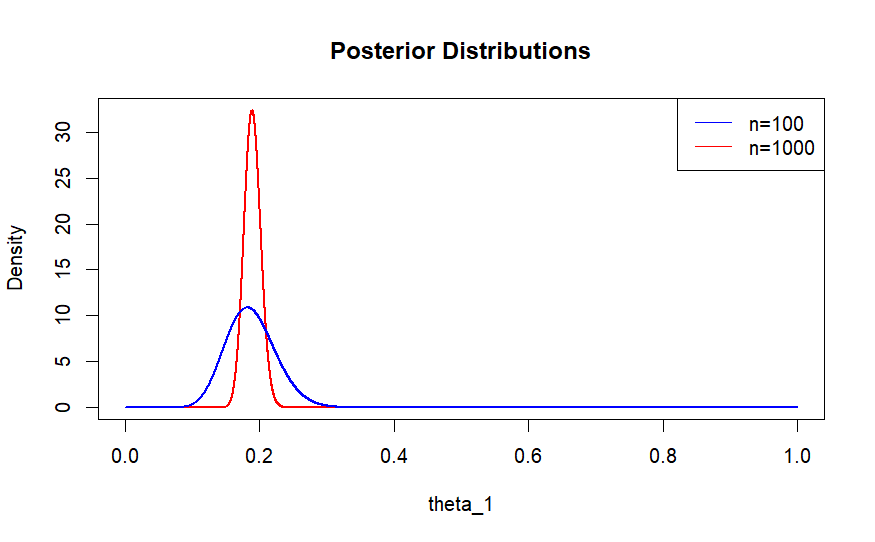
\includegraphics[width=0.7\textwidth]{Posterior_Distribution.png}
    \caption{Resulting Posterior Distributions of \(\theta_1\) for \(n = 100\) and \(n = 1000\)}
    \label{fig:myimage}
\end{figure}

From the plots we can clearly observe that the posterior distribution for \(n = 1000\) is much more concentrated at around 0.19 \( \left(= \frac{19}{100} = \frac{190}{1000}\right)\) then the posterior distribution for \(n=100\).

\subsection*{Effect of having a larger sample size}
As the sample size increases, the likelihood function (which represents the information from the data) becomes increasingly dominant over the prior distribution (which represents our initial beliefs).

With larger samples, the posterior distribution tends to become more concentrated around the true value of the parameter being estimated.
This concentration reflects the increased certainty that comes with more data.
The variance of the posterior distribution decreases, indicating a narrower range of plausible values for the parameter.


\newpage

\section*{Question 4}
Given \(Y_i (i = 1,\cdots, n)\) are i.i.d EXP(\(\theta\)), where the pdf of \(y\) is given by,
\[f(y_i|\theta) = \frac{1}{\theta} \exp(-\frac{y_i}{\theta})\]

\subsection*{Part(a)}
Jeffrey's prior for \(\theta\) is the square root of the information number of \(\theta\), \(I(\theta)\).

Now,
\begin{align*}
    I(\theta) &= E \left[\left(\frac{\partial}{\partial \theta } \log(f(y|\theta))\right)^2\right]\\
    &= E \left[\left(\frac{\partial}{\partial \theta } \log\left(\frac{1}{\theta}\exp\left(\frac{-y}{\theta}\right)\right)\right)^2\right] \\
    &=E \left[\left(\frac{\partial}{\partial \theta }\left(-\log\theta- \frac{y}{\theta}\right)\right)^2\right]\\
    &=E \left[\left(-\frac{1}{\theta}+ \frac{y}{\theta^2}\right)^2\right]\\
    &=E \left[\frac{1}{\theta^2} - 2\frac{y}{\theta^3} + \frac{y^2}{\theta^4}\right]\\
    &= \frac{1}{\theta^2} - \frac{2}{\theta^3} E[y] + \frac{1}{\theta^4} E[y^2]\\
    &= \frac{1}{\theta^2} - \frac{2}{\theta^3} \theta + \frac{1}{\theta^4} 2\theta^2\\
    &= \frac{1}{\theta^2}
\end{align*}

Therefore, the Jeffrey's prior for \(\theta\) is,
\begin{align*}
    \pi(\theta) &\propto \sqrt{I(\theta)}\\
    &\propto \sqrt{\frac{1}{\theta^2}}\\
    &\propto \frac{1}{\theta}
\end{align*}

\subsection*{Part(b)}
For \(\alpha = \theta^{-1}\), the pdf of \(y\) can be written as 
\[
    f(y|\alpha) = \alpha \exp(-\alpha y)
\]
The information number of \(\alpha\) is 
\begin{align*}
    I(\alpha) &= E \left[\left(\frac{\partial}{\partial \theta } \log(f(y|\alpha))\right)^2\right]\\
    &= E \left[\left(\frac{\partial}{\partial \alpha } \log\left(\alpha\exp\left(-\alpha y\right)\right)\right)^2\right]\\
    &= E \left[\left(\frac{1}{\alpha} -y \right)^2\right]\\
    &= E \left[\frac{1}{\alpha^2} -2 \frac{y}{\alpha} + y^2\right]\\
    &= \frac{1}{\alpha^2} - \frac{2}{\alpha} E[y] + E[y^2]\\
    &= \frac{1}{\alpha^2} - \frac{2}{\alpha^2} + \frac{2}{\alpha^2}\\
    &= \frac{1}{\alpha^2}
\end{align*}

Therefore, the Jeffrey's prior for \(\alpha\) is,

\begin{align*}
    \pi(\alpha) &\propto \sqrt{I(\alpha)}\\
    &\propto \sqrt{\frac{1}{\alpha^2}}\\
    &\propto \frac{1}{\alpha}
\end{align*}

\subsection*{Part(c)}

The posterior density of \(\theta\) corresponding to the prior density in (a) is,

\begin{align*}
    \pi(\theta|y) &\propto \left(\prod_{i=1}^{n}\frac{1}{\theta}\exp\left(-\frac{y_i}{\theta}\right)\right) \times \frac{1}{\theta}\\
    &\propto \frac{1}{\theta^{n+1}}\exp\left(-\frac{1}{\theta}\sum_{i=1}^{n}y_i\right)
\end{align*}

Where the last expression is the kernel of a Inverse Gamma distribution with shape parameter \(n\) and scale parameter \(\sum_{i=1}^{n}y_i\).

So, the posterior distribution of \(\theta\) is \(\text{IG}(n,\sum_{i=1}^{n}y_i)\).

\newpage

\section*{Question 5}
We are given the multiple linear regression model
\[y_i = x'_i\beta + \epsilon_i,\] 
where \(\epsilon_i|x_i\sim N(0,\sigma^2)\) for all \(i=1,\cdots,n\). The priors on \((\beta,\sigma^2)\) are independent and \(\pi(\beta, \sigma^2) = \pi(\beta)\pi(\sigma^2) = N_k(\beta_0,B_0)\text{IG}(\frac{\alpha_0}{2},\frac{\delta_0}{2})\).

\vspace{0.25cm}

Clearly, \(y_i \sim N(x'_i\beta, \sigma^2)\) for \(i = 1, \cdots, n\). So the likelihood is 
\begin{align*}
    f(y|\beta,\sigma^2) &= \prod_{i=1}^{n} \frac{1}{\sigma\sqrt{2\pi}}\exp\left(-\frac{(y_i - x'_i\beta)^2}{2\sigma^2}\right)\\
    &= (2\pi\sigma^2)^{-\frac{n}{2}}\exp\left(-\frac{1}{2\sigma^2}\sum_{i=1}^{n}(y_i - x'_i\beta)^2\right)\\
    &\propto \sigma^{-n}\exp\left(-\frac{1}{2\sigma^2}\sum_{i=1}^{n}(y_i - x'_i\beta)^2\right) = \sigma^{-n}\exp\left(-\frac{1}{2\sigma^2}(y - X\beta)'(y-X\beta)\right)
\end{align*}

So the posterior distribution of \((\beta,\sigma^2)\) is
\begin{align*}
    \pi(\beta,\sigma^2|y) &\propto f(y|\beta,\sigma^2)\pi(\beta,\sigma^2)\\
    &\propto f(y|\beta,\sigma^2)\pi(\beta)\pi(\sigma^2)\\
    &\propto \left(\frac{1}{\sigma^2}\right)^{\frac{n}{2}}\exp\left(-\frac{1}{2\sigma^2}(y - X\beta)'(y-X\beta)\right) \exp\left(-\frac{1}{2}(\beta - \beta_0)'B_0^{-1}(\beta - \beta_0)\right) \\
    &\quad \times \left(\frac{1}{\sigma^2}\right)^{\frac{\alpha_0}{2} + 1}\exp\left(-\frac{\delta_0}{2\sigma^2}\right)\\
    &\propto \left(\frac{1}{\sigma^2}\right)^{\frac{(n+\alpha_0)}{2}+1}\exp\left(-\frac{\delta_0}{2\sigma^2}\right)\exp\left(-\frac{1}{2\sigma^2}(y - X\beta)'(y-X\beta)\right) \\
    & \quad \times \exp\left(-\frac{1}{2}(\beta - \beta_0)'B_0^{-1}(\beta - \beta_0)\right)
\end{align*}


\subsection*{Part(a)}

We want to find $\pi(\beta | \sigma^2, y)$. We can ignore terms that don't involve $\beta$ in \(\pi(\beta,\sigma^2|y)\):
    \begin{align*}
        \pi(\beta | \sigma^2, y) &\propto \exp\left(-\frac{1}{2\sigma^2}(y - X\beta)'(y - X\beta)\right) \exp\left(-\frac{1}{2}(\beta - \beta_0)' B_0^{-1} (\beta - \beta_0)\right)\\
        &\propto \exp\left(-\frac{1}{2}\left(\frac{1}{\sigma^2}(y - X\beta)'(y - X\beta)+(\beta - \beta_0)' B_0^{-1} (\beta - \beta_0)\right)\right)
    \end{align*}
    
    Expand the quadratic terms :
    $$\frac{1}{\sigma^2}(y - X\beta)'(y - X\beta) = \frac{1}{\sigma^2}\left(\beta' X' X \beta - 2\beta' X' y + y'y\right) $$
    $$(\beta - \beta_0)' B_0^{-1} (\beta - \beta_0) = \beta' B_0^{-1} \beta - 2\beta' B_0^{-1} \beta_0 + \beta_0' B_0^{-1} \beta_0$$

    Adding the above two, we get:
    \begin{align*}
        \frac{1}{\sigma^2}(y - X\beta)'(y - X\beta)+(\beta - \beta_0)' B_0^{-1} (\beta - \beta_0) =  \beta' \left(\frac{1}{\sigma^2} X' X + B_0^{-1}\right) \beta - 2\beta'\left(\frac{1}{\sigma^2} X' y + B_0^{-1} \beta_0\right) \\
    + y'y + \beta_0'B_0^{-1}\beta_0
    \end{align*}


    Substituting this, we get:
    \begin{align*}
        \pi(\beta | \sigma^2, y) &\propto \exp\left(-\frac{1}{2} \left[ \beta' \left(\frac{1}{\sigma^2} X' X + B_0^{-1}\right) \beta - 2\beta'\left(\frac{1}{\sigma^2} X' y + B_0^{-1} \beta_0\right) + y'y + \beta_0'B_0^{-1}\beta_0 \right]\right)\\
        & \propto \exp\left(-\frac{1}{2} \left[ \beta' \left(\frac{1}{\sigma^2} X' X + B_0^{-1}\right) \beta - 2\beta' \left(\frac{1}{\sigma^2} X' y + B_0^{-1} \beta_0\right) \right] \right)
    \end{align*}

    Let $B_1^{-1} = \frac{1}{\sigma^2} X' X + B_0^{-1}$ and $\bar{\beta} = B_1 \left(\frac{1}{\sigma^2} X' y + B_0^{-1} \beta_0\right)$. Then:
    $$\pi(\beta | \sigma^2, y) \propto \exp\left(-\frac{1}{2} (\beta - \bar{\beta})' B_1^{-1} (\beta - \bar{\beta}) \right)$$
    So, the conditional posterior distribution of \(\beta\) is proportional to the kernel of the Normal distribution.

    Therefore, we have:
    $$\pi(\beta | \sigma^2, y) \sim N_k(\bar{\beta}, B_1)$$
    
    where $B_1 = \left(\frac{1}{\sigma^2} X' X + B_0^{-1}\right)^{-1}$ and $\bar{\beta} = B_1 \left(\frac{1}{\sigma^2} X' y + B_0^{-1} \beta_0\right)$.

\subsection*{Part(b)}

    We want to find $\pi(\sigma^2 | \beta, y)$. Again, ignore terms that don't involve $\sigma^2$:
   
    $$\pi(\sigma^2 | \beta, y) \propto \left(\frac{1}{\sigma^2}\right)^{\frac{\alpha_0 + n}{2} + 1} \exp\left(-\frac{1}{2\sigma^2} \left[ \delta_0 + (y - X\beta)'(y - X\beta) \right] \right)$$

    Let \(\alpha_1 = \alpha_0 + n\) and \(\delta_1 = \delta_0 + (y-X\beta)'(y-X\beta)\). Then:

    $$\pi(\sigma^2|\beta,y) \propto \left(\frac{1}{\sigma^2}\right)^{\frac{\alpha_1}{2}+1} \exp\left(-\frac{\delta_1}{2\sigma^2}\right)$$

    So the conditional posterior distribution of \(\sigma^2\) is proportional to the kernel of a Inverse Gamma distribution with shape parameter \(\frac{\alpha_1}{2}\) and scale parameter \(\frac{\delta_1}{2}\).
    Therefore, we have:
    $$\pi(\sigma^2 | \beta, y) \sim \text{IG}\left(\frac{\alpha_1}{2}, \frac{\delta_1}{2}\right)$$

\end{document}